% GNUPLOT: LaTeX picture with Postscript
\begingroup
  \makeatletter
  \providecommand\color[2][]{%
    \GenericError{(gnuplot) \space\space\space\@spaces}{%
      Package color not loaded in conjunction with
      terminal option `colourtext'%
    }{See the gnuplot documentation for explanation.%
    }{Either use 'blacktext' in gnuplot or load the package
      color.sty in LaTeX.}%
    \renewcommand\color[2][]{}%
  }%
  \providecommand\includegraphics[2][]{%
    \GenericError{(gnuplot) \space\space\space\@spaces}{%
      Package graphicx or graphics not loaded%
    }{See the gnuplot documentation for explanation.%
    }{The gnuplot epslatex terminal needs graphicx.sty or graphics.sty.}%
    \renewcommand\includegraphics[2][]{}%
  }%
  \providecommand\rotatebox[2]{#2}%
  \@ifundefined{ifGPcolor}{%
    \newif\ifGPcolor
    \GPcolortrue
  }{}%
  \@ifundefined{ifGPblacktext}{%
    \newif\ifGPblacktext
    \GPblacktexttrue
  }{}%
  % define a \g@addto@macro without @ in the name:
  \let\gplgaddtomacro\g@addto@macro
  % define empty templates for all commands taking text:
  \gdef\gplbacktext{}%
  \gdef\gplfronttext{}%
  \makeatother
  \ifGPblacktext
    % no textcolor at all
    \def\colorrgb#1{}%
    \def\colorgray#1{}%
  \else
    % gray or color?
    \ifGPcolor
      \def\colorrgb#1{\color[rgb]{#1}}%
      \def\colorgray#1{\color[gray]{#1}}%
      \expandafter\def\csname LTw\endcsname{\color{white}}%
      \expandafter\def\csname LTb\endcsname{\color{black}}%
      \expandafter\def\csname LTa\endcsname{\color{black}}%
      \expandafter\def\csname LT0\endcsname{\color[rgb]{1,0,0}}%
      \expandafter\def\csname LT1\endcsname{\color[rgb]{0,1,0}}%
      \expandafter\def\csname LT2\endcsname{\color[rgb]{0,0,1}}%
      \expandafter\def\csname LT3\endcsname{\color[rgb]{1,0,1}}%
      \expandafter\def\csname LT4\endcsname{\color[rgb]{0,1,1}}%
      \expandafter\def\csname LT5\endcsname{\color[rgb]{1,1,0}}%
      \expandafter\def\csname LT6\endcsname{\color[rgb]{0,0,0}}%
      \expandafter\def\csname LT7\endcsname{\color[rgb]{1,0.3,0}}%
      \expandafter\def\csname LT8\endcsname{\color[rgb]{0.5,0.5,0.5}}%
    \else
      % gray
      \def\colorrgb#1{\color{black}}%
      \def\colorgray#1{\color[gray]{#1}}%
      \expandafter\def\csname LTw\endcsname{\color{white}}%
      \expandafter\def\csname LTb\endcsname{\color{black}}%
      \expandafter\def\csname LTa\endcsname{\color{black}}%
      \expandafter\def\csname LT0\endcsname{\color{black}}%
      \expandafter\def\csname LT1\endcsname{\color{black}}%
      \expandafter\def\csname LT2\endcsname{\color{black}}%
      \expandafter\def\csname LT3\endcsname{\color{black}}%
      \expandafter\def\csname LT4\endcsname{\color{black}}%
      \expandafter\def\csname LT5\endcsname{\color{black}}%
      \expandafter\def\csname LT6\endcsname{\color{black}}%
      \expandafter\def\csname LT7\endcsname{\color{black}}%
      \expandafter\def\csname LT8\endcsname{\color{black}}%
    \fi
  \fi
    \setlength{\unitlength}{0.0500bp}%
    \ifx\gptboxheight\undefined%
      \newlength{\gptboxheight}%
      \newlength{\gptboxwidth}%
      \newsavebox{\gptboxtext}%
    \fi%
    \setlength{\fboxrule}{0.5pt}%
    \setlength{\fboxsep}{1pt}%
\begin{picture}(7200.00,5040.00)%
    \gplgaddtomacro\gplbacktext{%
      \csname LTb\endcsname%%
      \put(946,704){\makebox(0,0)[r]{\strut{}$4780$}}%
      \csname LTb\endcsname%%
      \put(946,998){\makebox(0,0)[r]{\strut{}$4785$}}%
      \csname LTb\endcsname%%
      \put(946,1292){\makebox(0,0)[r]{\strut{}$4790$}}%
      \csname LTb\endcsname%%
      \put(946,1586){\makebox(0,0)[r]{\strut{}$4795$}}%
      \csname LTb\endcsname%%
      \put(946,1880){\makebox(0,0)[r]{\strut{}$4800$}}%
      \csname LTb\endcsname%%
      \put(946,2174){\makebox(0,0)[r]{\strut{}$4805$}}%
      \csname LTb\endcsname%%
      \put(946,2468){\makebox(0,0)[r]{\strut{}$4810$}}%
      \csname LTb\endcsname%%
      \put(946,2762){\makebox(0,0)[r]{\strut{}$4815$}}%
      \csname LTb\endcsname%%
      \put(946,3055){\makebox(0,0)[r]{\strut{}$4820$}}%
      \csname LTb\endcsname%%
      \put(946,3349){\makebox(0,0)[r]{\strut{}$4825$}}%
      \csname LTb\endcsname%%
      \put(946,3643){\makebox(0,0)[r]{\strut{}$4830$}}%
      \csname LTb\endcsname%%
      \put(946,3937){\makebox(0,0)[r]{\strut{}$4835$}}%
      \csname LTb\endcsname%%
      \put(946,4231){\makebox(0,0)[r]{\strut{}$4840$}}%
      \csname LTb\endcsname%%
      \put(946,4525){\makebox(0,0)[r]{\strut{}$4845$}}%
      \csname LTb\endcsname%%
      \put(946,4819){\makebox(0,0)[r]{\strut{}$4850$}}%
      \csname LTb\endcsname%%
      \put(1078,484){\makebox(0,0){\strut{}$0$}}%
      \csname LTb\endcsname%%
      \put(1651,484){\makebox(0,0){\strut{}$1$}}%
      \csname LTb\endcsname%%
      \put(2223,484){\makebox(0,0){\strut{}$2$}}%
      \csname LTb\endcsname%%
      \put(2796,484){\makebox(0,0){\strut{}$3$}}%
      \csname LTb\endcsname%%
      \put(3368,484){\makebox(0,0){\strut{}$4$}}%
      \csname LTb\endcsname%%
      \put(3941,484){\makebox(0,0){\strut{}$5$}}%
      \csname LTb\endcsname%%
      \put(4513,484){\makebox(0,0){\strut{}$6$}}%
      \csname LTb\endcsname%%
      \put(5086,484){\makebox(0,0){\strut{}$7$}}%
      \csname LTb\endcsname%%
      \put(5658,484){\makebox(0,0){\strut{}$8$}}%
      \csname LTb\endcsname%%
      \put(6231,484){\makebox(0,0){\strut{}$9$}}%
      \csname LTb\endcsname%%
      \put(6803,484){\makebox(0,0){\strut{}$10$}}%
    }%
    \gplgaddtomacro\gplfronttext{%
      \csname LTb\endcsname%%
      \put(198,2761){\rotatebox{-270}{\makebox(0,0){\strut{}voltage / mV}}}%
      \csname LTb\endcsname%%
      \put(3940,154){\makebox(0,0){\strut{}resistor Rx / Ohm}}%
      \csname LTb\endcsname%%
      \put(3940,4709){\makebox(0,0){\strut{}}}%
      \put(132,-110){\makebox(0,0)[l]{\strut{}}}%
      \put(5517,4646){\makebox(0,0){\strut{}}}%
      \csname LTb\endcsname%%
      \put(5816,4646){\makebox(0,0)[r]{\strut{}PC0, type 2}}%
    }%
    \gplbacktext
    \put(0,0){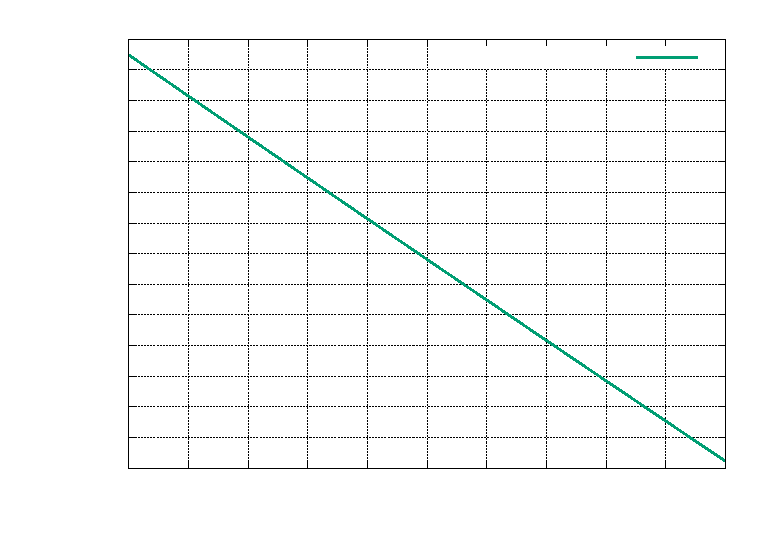
\includegraphics{../GNU/RLvhigh}}%
    \gplfronttext
  \end{picture}%
\endgroup
